\begin{figure}[!t]
	\centering
	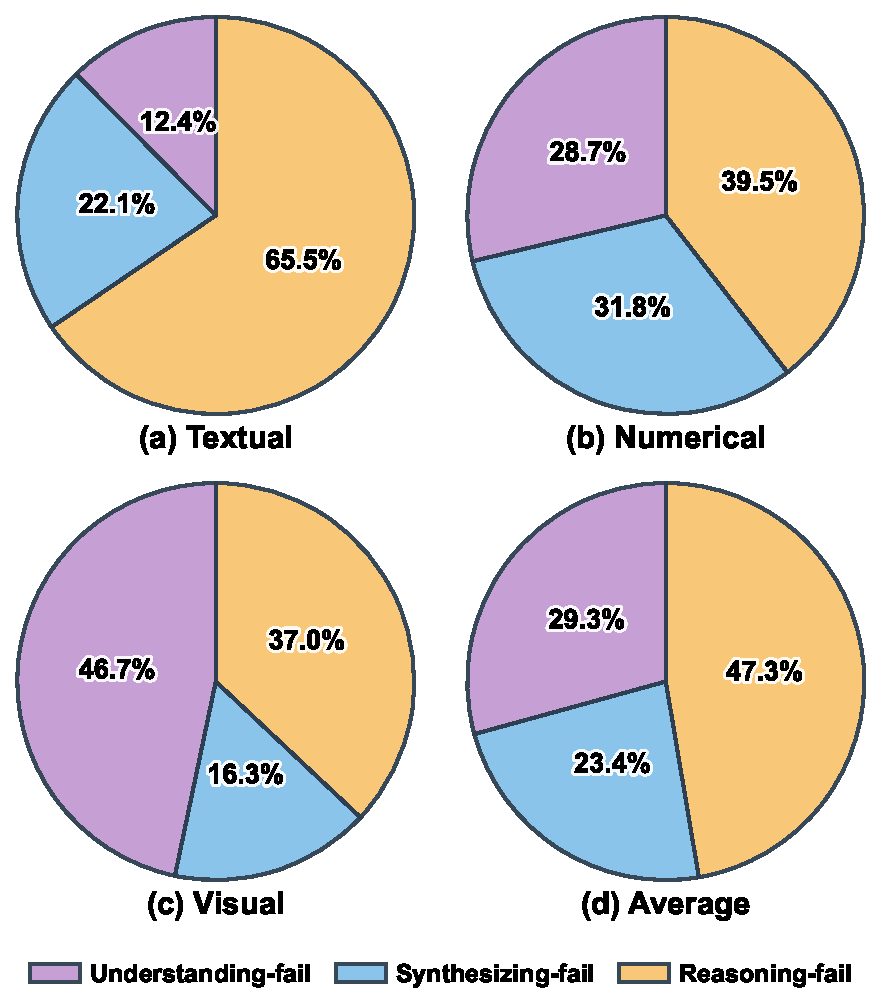
\includegraphics[width=0.90\linewidth]{figure/figure15.pdf}
	\caption{Error Attribution across the U/S/R Chain, exposing the fragility of High-Level Cognition in LLMs.}
	\label{fig:HCL}
\end{figure}

\section{Discussion}
\label{sec:discussion}

This section fundamentally and insightfully explores the underlying mechanisms of this collapse and its implications for future real Artificial General Intelligence (AGI). 

Specifically, we deconstruct the collapse into deficits across \textbf{three core characteristics}: 
(i) the \emph{violation of Modality-Agnosticism}, evaluated via cross-modal performance comparisons; 
(ii) the \emph{breakdown of High-Level Cognition}, analyzed through error attribution along the Understanding-Synthesizing-Reasoning (U/S/R) chain; 
and (iii) the \emph{absence of Open-ended Evolution}, demonstrated by contrasting general LMs, fine-tuned LMs, and traditional architectures. 
% Furthermore, we stress-test the models using few-shot learning to rule out shallow causes like insufficient context. 
Finally, we highlight the \textbf{evolutionary bottlenecks} in the current AGI trajectory and outline future directions.

\begin{figure}[!t]
	\centering
	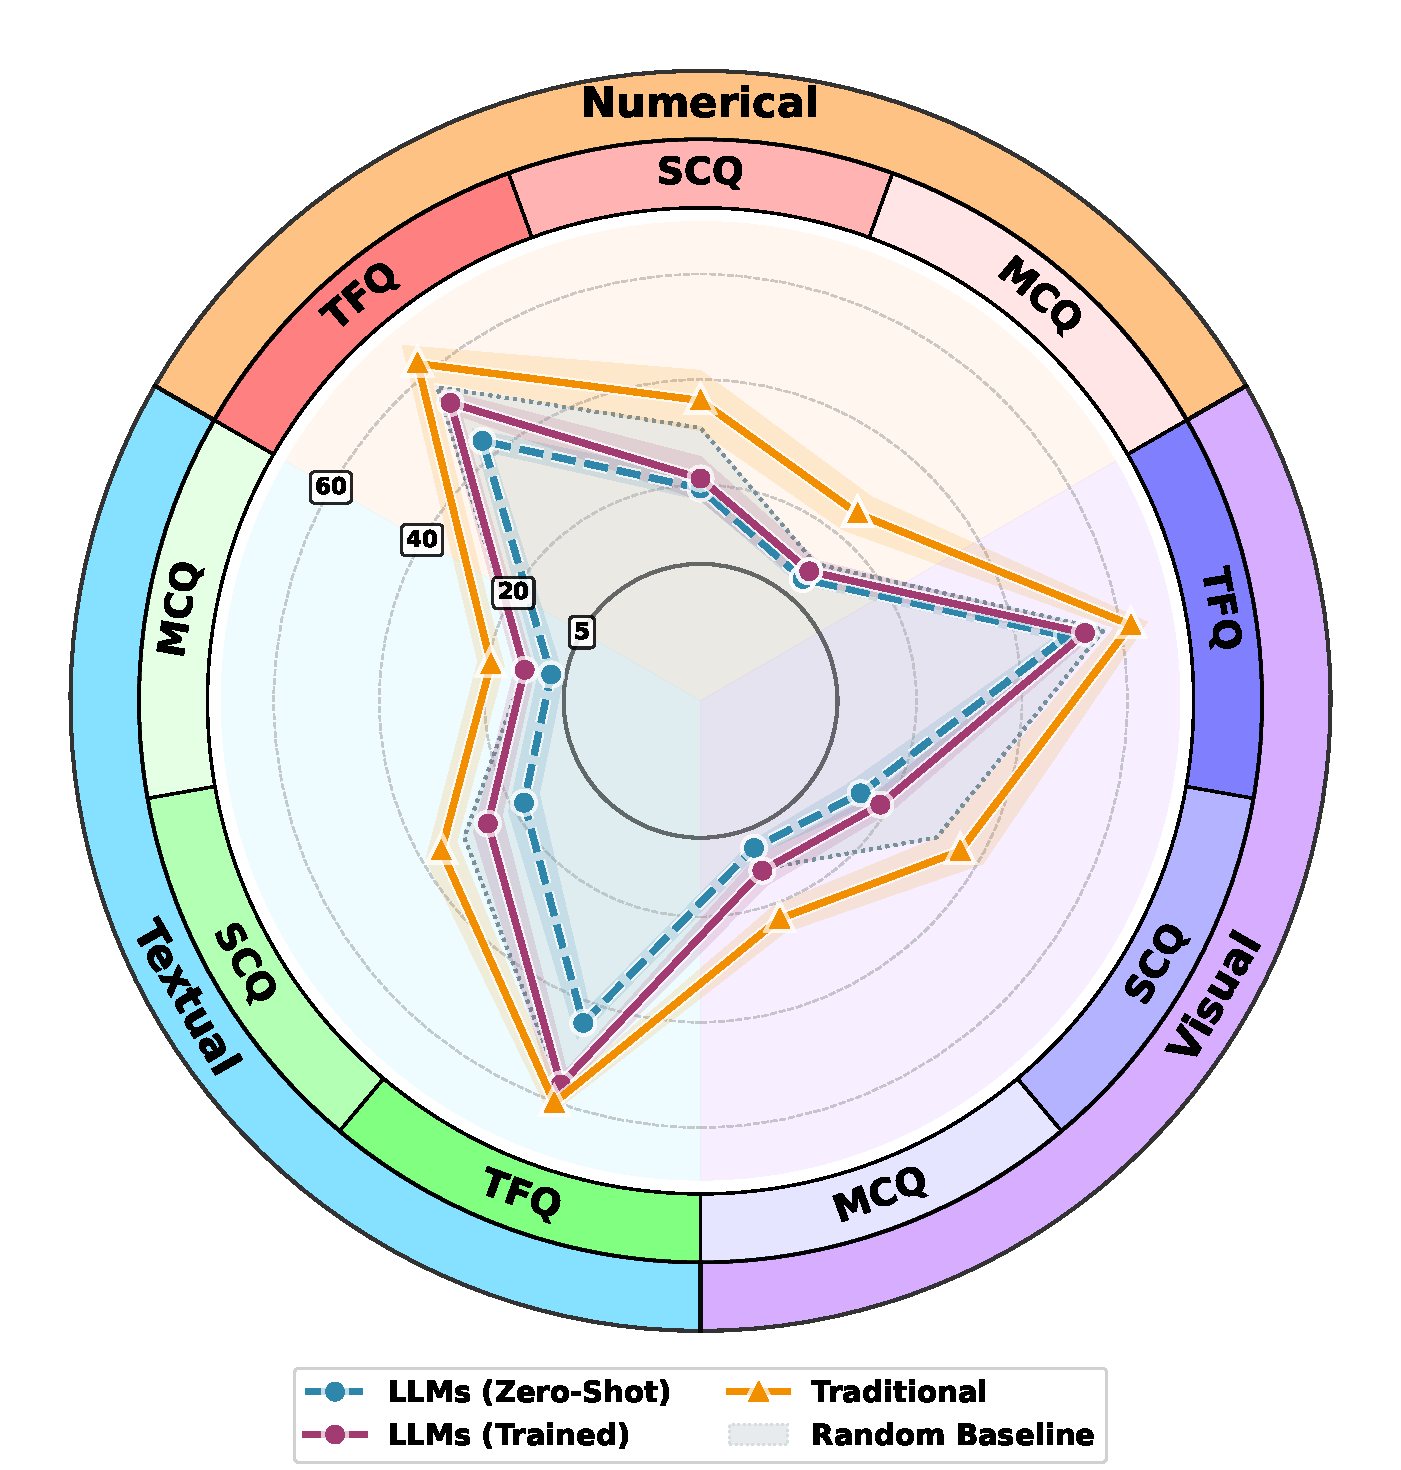
\includegraphics[width=\linewidth]{figure/figure18.pdf}
	\vspace{-5mm}
    \caption{Evaluation of Open-Ended Evolution comparing LLMs and traditional-architecture models across modalities.}
    \vspace{-4mm}
	\label{fig:evolution}
\end{figure}

\subsection{Modality-Agnosticism}
\label{modality}

To evaluate the \textit{Modality-Agnostic} capability, we analyze performance across different modalities with various problem tasks illustrated in Figure ~\ref{fig:cross-modality}. 

While elite models maintain a fragile reasoning facade in the textual modality, their cognitive capabilities catastrophically collapse in \emph{non-semantic environments}.
Remarkably, massive LLMs universally perform \emph{worse than random chance} across all metrics. 
The most glaring deficit occurs in the simplest binary task (TFQ, random baseline $56.74\%^\dagger$), where models like LLaVa-1.5 (Visual) and Vicuna-1.5 (Numerical) plunge to a mere $50.00\%$. 
As reasoning complexity increases, the capability gap widens to absurd proportions: on the visual MCQ, LLaVa-1.5 yields just $5.40\%$, and Llama-3.1 (70B) scores a dismal $6.40\%$ on the numerical MCQ. 
% Both scores are less than half the $12.95\%^\dagger$ random baseline. 
This multi-dimensional, sub-random collapse definitively proves that current LMs \textbf{lack genuine modality-agnosticism}; their reasoning is heavily tethered to textual semantic shortcuts, completely failing to integrate raw physical signals.
In stark contrast, specialized lightweight traditional-architecture models provide compelling empirical proof for representational equivalence. 
Despite processing radically different raw inputs, these models not only overwhelmingly crush their billion-parameter counterparts but also converge on nearly identical predictive distributions. 

This gap indicates that the next frontier of AGI is not simply scaling language priors, but \textbf{learning abstractions that remain invariant across how the world is observed}. 
If future models cannot reason consistently beyond text, then their apparent intelligence may remain a semantic illusion rather than genuine world intelligence.

% Whether utilizing a Textual GRU, a Numerical CNN, or a Visual EfficientNet-B0, their accuracies universally stabilize across the entire gradient: 
% peaking at $60\%$-$63\%$ on TFQ, $32\%$-$38\%$ on SCQ, and $19\%$-$25\%$ on MCQ. 
% This flawless tri-modal convergence confirms that objective physical truths are invariant to sensory channels. 
% It proves that once a model's architecture aligns with the physical world's structural logic, it can consistently extract identical macroscopic laws regardless of the data modality.

\begin{figure*}[!t]
	\centering
	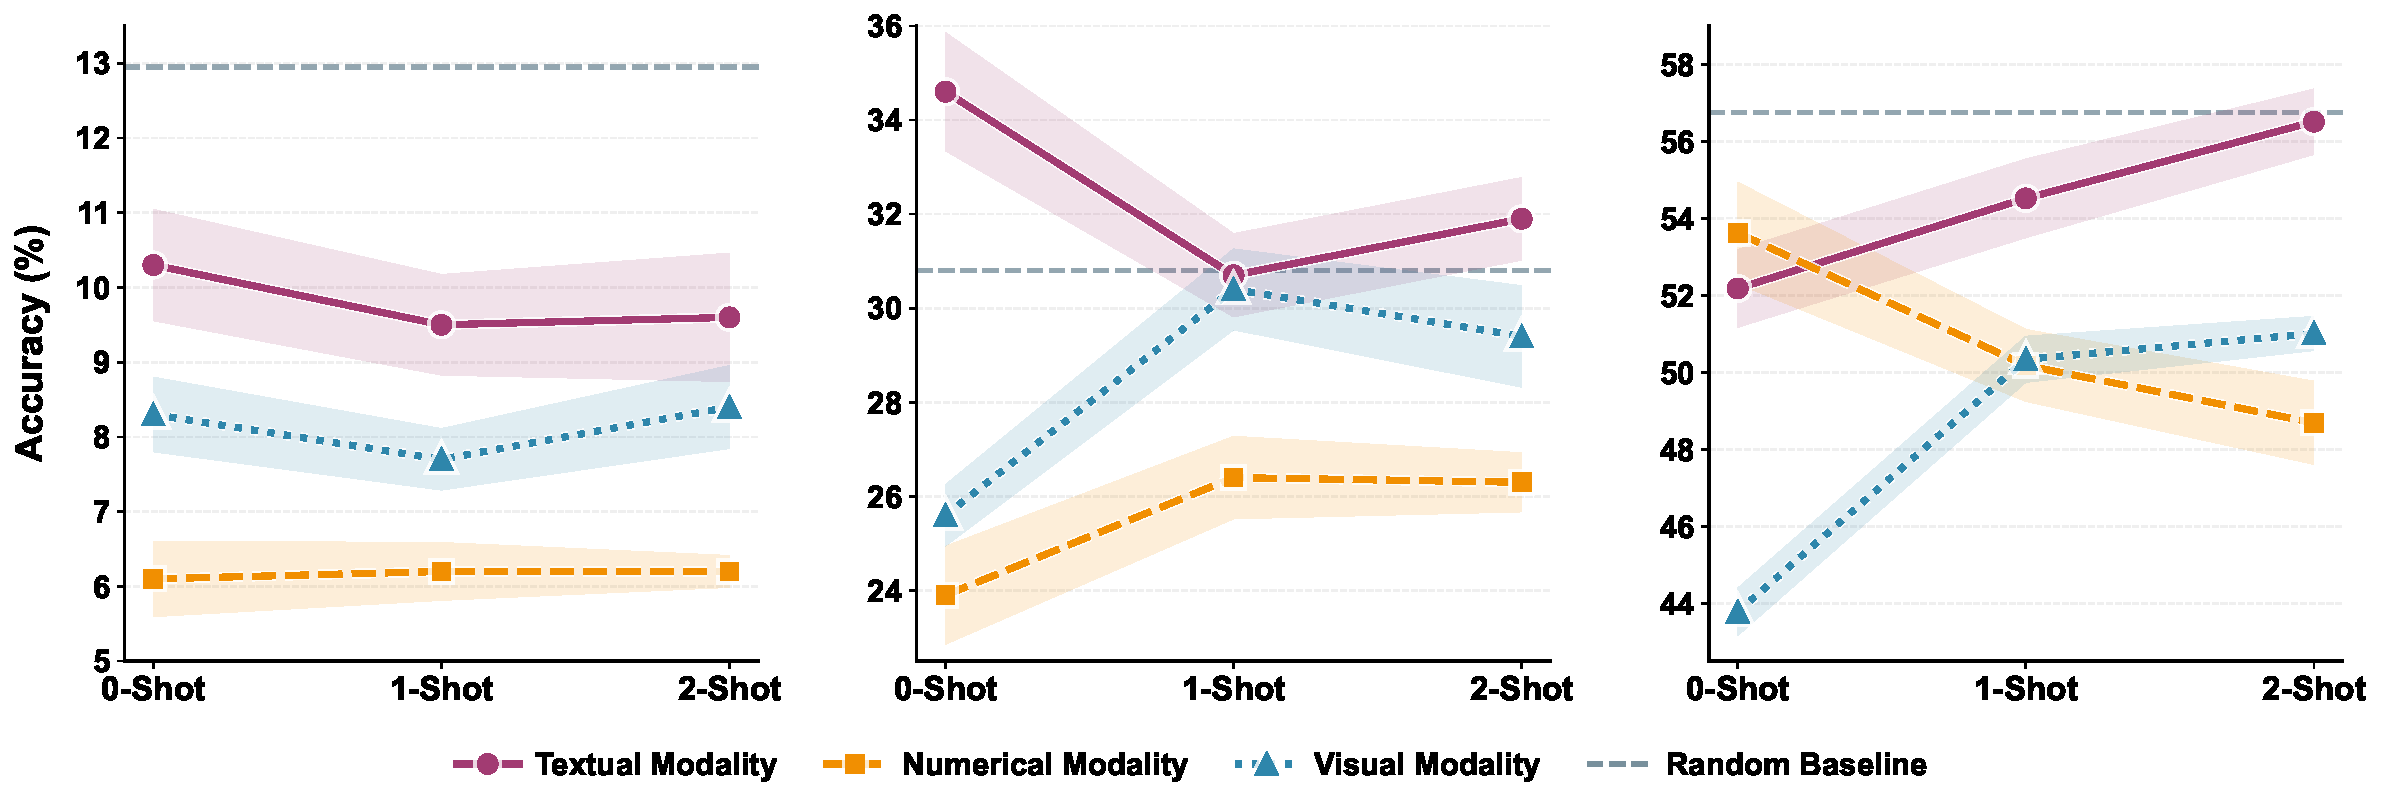
\includegraphics[width=\linewidth]{figure/figure16.pdf}
    \vspace{-5mm}
	\caption{Few-Shot Learning (FSL) Stress-Test. Accuracy trajectories across 0, 1, and 2-shot settings. Flat or degrading performance near random baselines indicates that FSL fails to trigger endogenous cognitive reasoning. (From left to right: MCQ, SCQ, TFQ)}
    \vspace{-2mm}
	\label{fig:few_shot_ablation}
\end{figure*}

\subsection{High-Level Cognition}
\label{HLC}

To gain deeper insight into the cognitive bottlenecks of High-Level Cognition for LLMs, we decompose each incorrect response by identifying its most probable point of failure within the U/S/R pipeline across modalities in Figure ~\ref{fig:HCL}, following the criteria detailed in Appendix~\ref{sec:usrules}. 

This diagnostic perspective serves as a vital complement to holistic accuracy: it reveals that models with comparable performance may nonetheless exhibit fundamentally distinct failure modes, exposing unique fractures along their internal cognitive chains. 
In the \emph{textual} modality, the majority of errors ($65.5\%$) are concentrated in the Reasoning stage. 
This suggests that while LLMs can maintain a facade of Understanding by adhering to output constraints (low U-fail), they lack the underlying world model to execute correct physical deduction. 
Meanwhile, as we shift to the \emph{numerical} and \emph{visual} modalities, we observe a surge in U-fail (reaching $46.7\%$ in visual tasks). 
This indicates that raw physical signals act as representational noise that disrupts the models' instruction-following stability, causing them to abandon the requested output formats entirely. 
Furthermore, the high S-fail in the \emph{numerical} modality ($31.8\%$) reflects a profound internal logical dissonance, where models simultaneously generate mutually exclusive physical states. 

These findings suggest that the next frontier for LLM research is not merely improving answer accuracy, but building models whose \textbf{cognitive pipelines remain structurally coherent} even when reasoning must emerge directly from raw world signals rather than semantic shortcuts.


\subsection{Open-Ended Evolution}
\label{evolution}
Facing specific physical-world problems, the training process of the model essentially serves as a mechanism to approximate the performance upper bound for a given task.

Empirical results in Figure ~\ref{fig:evolution} demonstrate that traditional architecture models establish a stable performance baseline through training, representing the physical upper bound of the \emph{passive fitting} capacity on specific data distributions within traditional AI paradigms. 
However, a compelling phenomenon emerges: 
despite undergoing equivalent training regimes, LLMs not only fail to surpass but comprehensively underperform compared to traditional architecture models. 
This performance therefore inversion exposes profound architectural limitations within LLMs: 
they are fundamentally incapable of efficiently achieving passive fitting to specific physical dynamics, even within closed environments. 

Following an a fortiori argument, Open-ended Evolution requires an intelligent agent to \textbf{continuously assimilate and reorganize knowledge} through active interaction with complex physical environments. 
If current LLMs fail even to reach the upper bound of passive fitting in closed settings, then their limitation is not merely insufficient training, but a more fundamental mismatch between next-token prediction and genuine cognitive evolution. 


\subsection{Exploration and Future Work}
\label{future}

To investigate whether the observed collapse partially stems from the lack of task-specific context, we conducted a rigorous stress-test using \textbf{Few-Shot Learning} (FSL) with 1-shot and 2-shot demonstrations. 
The empirical results reveal a profound stagnation in capability emergence. Despite providing explicit examples, model performance remains stubbornly tethered to the mathematical random baseline. 
% In the numerical modality, for instance, MCQ accuracy remained virtually frozen at approximately $6.20\%$. Most strikingly, in the textual modality, increasing demonstrations to 2-shot actually led to a marginal performance decline (from $10.30\%$ to $9.60\%$). 
Qualitative analysis of the error logs also confirms that while FSL marginally improves template compliance and reducing Understanding-fail pattern, it still fails to trigger any substantive reduction in Reasoning-fail pattern with exacerbated reasoning errors. 
To summarize, this decoupling proves that FSL in current LLMs provides only \textbf{surface-level alignment} instead of perceiving the underlying laws of the physical world. 

Taken together, the failures across \textbf{modality, cognition, and evolution} indicate that current LLMs are constrained by a \emph{paradigm that remains fundamentally text-bound, externally scaffolded, and passively optimized}. 
The next stage of AGI will therefore require a shift from scaling semantic prediction to building systems that can \emph{form unified world representations, maintain endogenous cognitive structure, and grow through real interaction}. 
Under this view, HWI defines a broader transition for the field: from language competence toward authentic world intelligence.

% In the absence of genuine physical logic, additional context acts as "semantic noise" that further destabilizes the model’s fragile reasoning. 
% This decoupling proves that FSL in current LLMs provides only surface-level alignment; it teaches the model how to output a response without enabling the structural cognitive required to perceive the underlying laws of the physical world. 
% Consequently, the persistence of sub-random performance across all shot settings exposes an insurmountable capability ceiling within the "autoregressive next-token prediction" paradigm. 
% These findings demonstrate that AGI cannot be realized through prompt engineering or scaling context alone; it necessitates a paradigm shift toward an endogenous, modality-agnostic architecture capable of autonomous, world-oriented synthesis.
